\documentclass{lab1-article}

\title{Caduta di un grave}

\usepackage{fancyvrb}
\usepackage{hyperref}
\makeatletter
\def\PY@reset{\let\PY@it=\relax \let\PY@bf=\relax%
    \let\PY@ul=\relax \let\PY@tc=\relax%
    \let\PY@bc=\relax \let\PY@ff=\relax}
\def\PY@tok#1{\csname PY@tok@#1\endcsname}
\def\PY@toks#1+{\ifx\relax#1\empty\else%
    \PY@tok{#1}\expandafter\PY@toks\fi}
\def\PY@do#1{\PY@bc{\PY@tc{\PY@ul{%
    \PY@it{\PY@bf{\PY@ff{#1}}}}}}}
\def\PY#1#2{\PY@reset\PY@toks#1+\relax+\PY@do{#2}}

\expandafter\def\csname PY@tok@gd\endcsname{\def\PY@tc##1{\textcolor[rgb]{0.63,0.00,0.00}{##1}}}
\expandafter\def\csname PY@tok@gu\endcsname{\let\PY@bf=\textbf\def\PY@tc##1{\textcolor[rgb]{0.50,0.00,0.50}{##1}}}
\expandafter\def\csname PY@tok@gt\endcsname{\def\PY@tc##1{\textcolor[rgb]{0.00,0.27,0.87}{##1}}}
\expandafter\def\csname PY@tok@gs\endcsname{\let\PY@bf=\textbf}
\expandafter\def\csname PY@tok@gr\endcsname{\def\PY@tc##1{\textcolor[rgb]{1.00,0.00,0.00}{##1}}}
\expandafter\def\csname PY@tok@cm\endcsname{\let\PY@it=\textit\def\PY@tc##1{\textcolor[rgb]{0.25,0.50,0.50}{##1}}}
\expandafter\def\csname PY@tok@vg\endcsname{\def\PY@tc##1{\textcolor[rgb]{0.10,0.09,0.49}{##1}}}
\expandafter\def\csname PY@tok@m\endcsname{\def\PY@tc##1{\textcolor[rgb]{0.40,0.40,0.40}{##1}}}
\expandafter\def\csname PY@tok@mh\endcsname{\def\PY@tc##1{\textcolor[rgb]{0.40,0.40,0.40}{##1}}}
\expandafter\def\csname PY@tok@go\endcsname{\def\PY@tc##1{\textcolor[rgb]{0.53,0.53,0.53}{##1}}}
\expandafter\def\csname PY@tok@ge\endcsname{\let\PY@it=\textit}
\expandafter\def\csname PY@tok@vc\endcsname{\def\PY@tc##1{\textcolor[rgb]{0.10,0.09,0.49}{##1}}}
\expandafter\def\csname PY@tok@il\endcsname{\def\PY@tc##1{\textcolor[rgb]{0.40,0.40,0.40}{##1}}}
\expandafter\def\csname PY@tok@cs\endcsname{\let\PY@it=\textit\def\PY@tc##1{\textcolor[rgb]{0.25,0.50,0.50}{##1}}}
\expandafter\def\csname PY@tok@cp\endcsname{\def\PY@tc##1{\textcolor[rgb]{0.74,0.48,0.00}{##1}}}
\expandafter\def\csname PY@tok@gi\endcsname{\def\PY@tc##1{\textcolor[rgb]{0.00,0.63,0.00}{##1}}}
\expandafter\def\csname PY@tok@gh\endcsname{\let\PY@bf=\textbf\def\PY@tc##1{\textcolor[rgb]{0.00,0.00,0.50}{##1}}}
\expandafter\def\csname PY@tok@ni\endcsname{\let\PY@bf=\textbf\def\PY@tc##1{\textcolor[rgb]{0.60,0.60,0.60}{##1}}}
\expandafter\def\csname PY@tok@nl\endcsname{\def\PY@tc##1{\textcolor[rgb]{0.63,0.63,0.00}{##1}}}
\expandafter\def\csname PY@tok@nn\endcsname{\let\PY@bf=\textbf\def\PY@tc##1{\textcolor[rgb]{0.00,0.00,1.00}{##1}}}
\expandafter\def\csname PY@tok@no\endcsname{\def\PY@tc##1{\textcolor[rgb]{0.53,0.00,0.00}{##1}}}
\expandafter\def\csname PY@tok@na\endcsname{\def\PY@tc##1{\textcolor[rgb]{0.49,0.56,0.16}{##1}}}
\expandafter\def\csname PY@tok@nb\endcsname{\def\PY@tc##1{\textcolor[rgb]{0.00,0.50,0.00}{##1}}}
\expandafter\def\csname PY@tok@nc\endcsname{\let\PY@bf=\textbf\def\PY@tc##1{\textcolor[rgb]{0.00,0.00,1.00}{##1}}}
\expandafter\def\csname PY@tok@nd\endcsname{\def\PY@tc##1{\textcolor[rgb]{0.67,0.13,1.00}{##1}}}
\expandafter\def\csname PY@tok@ne\endcsname{\let\PY@bf=\textbf\def\PY@tc##1{\textcolor[rgb]{0.82,0.25,0.23}{##1}}}
\expandafter\def\csname PY@tok@nf\endcsname{\def\PY@tc##1{\textcolor[rgb]{0.00,0.00,1.00}{##1}}}
\expandafter\def\csname PY@tok@si\endcsname{\let\PY@bf=\textbf\def\PY@tc##1{\textcolor[rgb]{0.73,0.40,0.53}{##1}}}
\expandafter\def\csname PY@tok@s2\endcsname{\def\PY@tc##1{\textcolor[rgb]{0.73,0.13,0.13}{##1}}}
\expandafter\def\csname PY@tok@vi\endcsname{\def\PY@tc##1{\textcolor[rgb]{0.10,0.09,0.49}{##1}}}
\expandafter\def\csname PY@tok@nt\endcsname{\let\PY@bf=\textbf\def\PY@tc##1{\textcolor[rgb]{0.00,0.50,0.00}{##1}}}
\expandafter\def\csname PY@tok@nv\endcsname{\def\PY@tc##1{\textcolor[rgb]{0.10,0.09,0.49}{##1}}}
\expandafter\def\csname PY@tok@s1\endcsname{\def\PY@tc##1{\textcolor[rgb]{0.73,0.13,0.13}{##1}}}
\expandafter\def\csname PY@tok@sh\endcsname{\def\PY@tc##1{\textcolor[rgb]{0.73,0.13,0.13}{##1}}}
\expandafter\def\csname PY@tok@sc\endcsname{\def\PY@tc##1{\textcolor[rgb]{0.73,0.13,0.13}{##1}}}
\expandafter\def\csname PY@tok@sx\endcsname{\def\PY@tc##1{\textcolor[rgb]{0.00,0.50,0.00}{##1}}}
\expandafter\def\csname PY@tok@bp\endcsname{\def\PY@tc##1{\textcolor[rgb]{0.00,0.50,0.00}{##1}}}
\expandafter\def\csname PY@tok@c1\endcsname{\let\PY@it=\textit\def\PY@tc##1{\textcolor[rgb]{0.25,0.50,0.50}{##1}}}
\expandafter\def\csname PY@tok@kc\endcsname{\let\PY@bf=\textbf\def\PY@tc##1{\textcolor[rgb]{0.00,0.50,0.00}{##1}}}
\expandafter\def\csname PY@tok@c\endcsname{\let\PY@it=\textit\def\PY@tc##1{\textcolor[rgb]{0.25,0.50,0.50}{##1}}}
\expandafter\def\csname PY@tok@mf\endcsname{\def\PY@tc##1{\textcolor[rgb]{0.40,0.40,0.40}{##1}}}
\expandafter\def\csname PY@tok@err\endcsname{\def\PY@bc##1{\setlength{\fboxsep}{0pt}\fcolorbox[rgb]{1.00,0.00,0.00}{1,1,1}{\strut ##1}}}
\expandafter\def\csname PY@tok@kd\endcsname{\let\PY@bf=\textbf\def\PY@tc##1{\textcolor[rgb]{0.00,0.50,0.00}{##1}}}
\expandafter\def\csname PY@tok@ss\endcsname{\def\PY@tc##1{\textcolor[rgb]{0.10,0.09,0.49}{##1}}}
\expandafter\def\csname PY@tok@sr\endcsname{\def\PY@tc##1{\textcolor[rgb]{0.73,0.40,0.53}{##1}}}
\expandafter\def\csname PY@tok@mo\endcsname{\def\PY@tc##1{\textcolor[rgb]{0.40,0.40,0.40}{##1}}}
\expandafter\def\csname PY@tok@kn\endcsname{\let\PY@bf=\textbf\def\PY@tc##1{\textcolor[rgb]{0.00,0.50,0.00}{##1}}}
\expandafter\def\csname PY@tok@mi\endcsname{\def\PY@tc##1{\textcolor[rgb]{0.40,0.40,0.40}{##1}}}
\expandafter\def\csname PY@tok@gp\endcsname{\let\PY@bf=\textbf\def\PY@tc##1{\textcolor[rgb]{0.00,0.00,0.50}{##1}}}
\expandafter\def\csname PY@tok@o\endcsname{\def\PY@tc##1{\textcolor[rgb]{0.40,0.40,0.40}{##1}}}
\expandafter\def\csname PY@tok@kr\endcsname{\let\PY@bf=\textbf\def\PY@tc##1{\textcolor[rgb]{0.00,0.50,0.00}{##1}}}
\expandafter\def\csname PY@tok@s\endcsname{\def\PY@tc##1{\textcolor[rgb]{0.73,0.13,0.13}{##1}}}
\expandafter\def\csname PY@tok@kp\endcsname{\def\PY@tc##1{\textcolor[rgb]{0.00,0.50,0.00}{##1}}}
\expandafter\def\csname PY@tok@w\endcsname{\def\PY@tc##1{\textcolor[rgb]{0.73,0.73,0.73}{##1}}}
\expandafter\def\csname PY@tok@kt\endcsname{\def\PY@tc##1{\textcolor[rgb]{0.69,0.00,0.25}{##1}}}
\expandafter\def\csname PY@tok@ow\endcsname{\let\PY@bf=\textbf\def\PY@tc##1{\textcolor[rgb]{0.67,0.13,1.00}{##1}}}
\expandafter\def\csname PY@tok@sb\endcsname{\def\PY@tc##1{\textcolor[rgb]{0.73,0.13,0.13}{##1}}}
\expandafter\def\csname PY@tok@k\endcsname{\let\PY@bf=\textbf\def\PY@tc##1{\textcolor[rgb]{0.00,0.50,0.00}{##1}}}
\expandafter\def\csname PY@tok@se\endcsname{\let\PY@bf=\textbf\def\PY@tc##1{\textcolor[rgb]{0.73,0.40,0.13}{##1}}}
\expandafter\def\csname PY@tok@sd\endcsname{\let\PY@it=\textit\def\PY@tc##1{\textcolor[rgb]{0.73,0.13,0.13}{##1}}}

\def\PYZbs{\char`\\}
\def\PYZus{\char`\_}
\def\PYZob{\char`\{}
\def\PYZcb{\char`\}}
\def\PYZca{\char`\^}
\def\PYZam{\char`\&}
\def\PYZlt{\char`\<}
\def\PYZgt{\char`\>}
\def\PYZsh{\char`\#}
\def\PYZpc{\char`\%}
\def\PYZdl{\char`\$}
\def\PYZhy{\char`\-}
\def\PYZsq{\char`\'}
\def\PYZdq{\char`\"}
\def\PYZti{\char`\~}
% for compatibility with earlier versions
\def\PYZat{@}
\def\PYZlb{[}
\def\PYZrb{]}
\makeatother


\begin{document}


\begin{article}
\selectlanguage{italian}

\maketitle

\secintro


Lo scopo dell'esperienza \`e lo studio della legge oraria di un corpo in caduta
libera analizzando un filmato registrato con lo \emph{smartphone}.

\secmaterialsdad

\begin{itemize}
\item Un grave\footnote{La cosa \`e probabilmente ovvia, ma scegliete un oggetto
  che: (i) non metta a repentaglio in alcun modo la vostra incolumit\`a;
  (ii) non rischi di danneggiare il pavimento o l'arredo;
  (iii) non rischi di rompersi cadendo.}.
\item Metro a nastro.
\item Smartphone o macchina fotografica digitale.
\end{itemize}


\secmeasurements

Misureremo, a tempi fissati, le posizioni dell'oggetto durante la caduta
analizzando i singoli fotogrammi del filmato realizzato con il nostro
\emph{smartphone}.

\begin{figure}[!htb]
  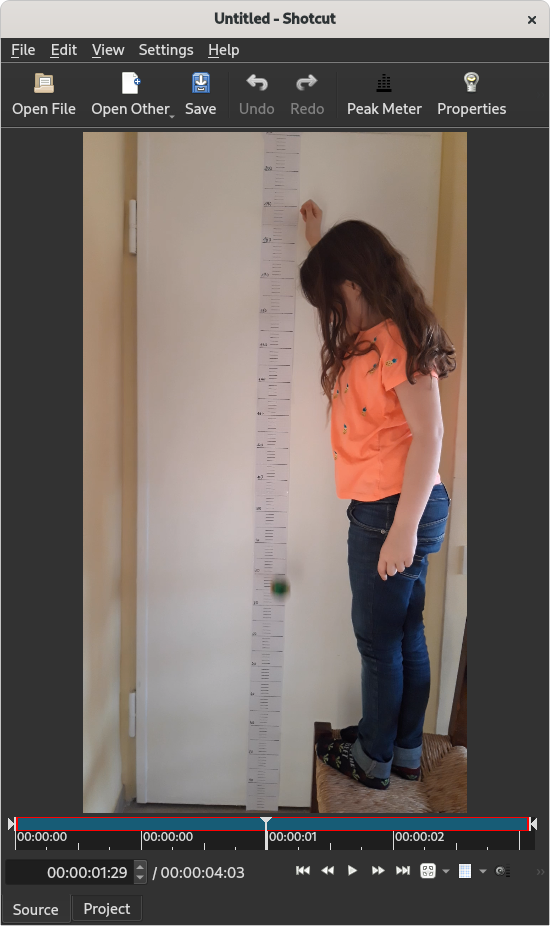
\includegraphics[width=\linewidth]{figures/caduta}
\end{figure}


Per fissare le idee, il tempo di caduta di un oggetto da un'altezza iniziale
$h_0 = 2$~m \`e
\begin{align*}
  t_0 = \sqrt{\frac{2h_0}{g}} \sim 0.64~\text{s},
\end{align*}
che, alla frequenza tipica di $30$~fotogrammi al secondo, ci permette di
campionare la caduta in almeno una ventina di punti.


\labsubsection{Analisi del file video}

Per analizzare il file video avrete bisogno di un \emph{editor} che vi permetta
di navigare i fotogrammi. Se non avere particolari preferenze,
\href{https://shotcut.org/}{Shotcut} \`e un \emph{editor open-source} e
multi-piattaforma che fa al caso vostro. (Ma la cosa \`e talmente semplice che
qualsiasi programa va bene.)

Il modo pi\`u semplice per misurare l'altezza dell'oggetto fotogramma
per fotogramma \`e quello di avere una guida centimetrata sullo sfondo,
come mostrato in figura.


\labsubsection{Fit della legge oraria}

Realizzate un grafico dell'altezza $h(t_i)$ in funzione dei tempi $t_i$ dei
fotogrammi interessanti (i.e., quelli in cui effettivamente l'oggetto sta
cadendo). Fittate il grafico di dispersione con una parabola
\begin{align}
  h(t) = \frac{1}{2}at^2 + v_0 t + h_0
\end{align}
confrontate il valore di \emph{best-fit} per l'accelerazione $a$ con
l'accelerazione di gravit\`a $g$.

Fate un grafico dei residui per valutare qualitativamente la bont\`a del modello.


\secconsiderations

Come vedete dalla figura, un fotogramma non \`e un immagine \emph{istantanea},
ma un integrale su un intervallo di tempo piccolo ma finito, per cui \`e
perfettamente normale che gli oggetti in movimento possano apparire sfuocati.
Nel nostro caso particolare, la cosa pu\`o avere impatto sulla stima dell'incertezza
di misura sulla posizione---che potenzialmente \`e maggiore quanto pi\`u velocemente
si muove l'oggetto.

Fate bene attenzione a come sono indicati i tempi dei frame nel programma
di \emph{editing} video che utilizzate per l'analisi: secondi con parte decimale,
indice del fotogramma oppure un misto? (Nella figura, ad esempio,
\texttt{00:00:01:29} significa: $0$ ore, $0$ minuti, $1$ secondo e $29$ fotogrammi.)
Va da s\'e che per passare da fotogrammi a frazione di secondo dovete dividere
per il \emph{frame rate} (tipicamente 30 fps), che \`e quindi importante sapere.

\onecolumn

\begin{Verbatim}[label=\makebox{\href{https://github.com/unipi-physics-labs/lab1-sheets/tree/main/snippy/dad_caduta.py}{https://github.com/.../dad\_caduta.py}},commandchars=\\\{\}]
\PY{k+kn}{import}\PY{+w}{ }\PY{n+nn}{numpy}\PY{+w}{ }\PY{k}{as}\PY{+w}{ }\PY{n+nn}{np}
\PY{k+kn}{from}\PY{+w}{ }\PY{n+nn}{matplotlib}\PY{+w}{ }\PY{k+kn}{import} \PY{n}{pyplot} \PY{k}{as} \PY{n}{plt}
\PY{k+kn}{from}\PY{+w}{ }\PY{n+nn}{scipy}\PY{n+nn}{.}\PY{n+nn}{optimize}\PY{+w}{ }\PY{k+kn}{import} \PY{n}{curve\PYZus{}fit}

\PY{c+c1}{\PYZsh{} Misure dirette\PYZhy{}\PYZhy{}\PYZhy{}mettete i vostri numeri!}
\PY{c+c1}{\PYZsh{} Qui potete anche leggere i dati da file, usando il metodo np.loadtxt(),}
\PY{c+c1}{\PYZsh{} se lo trovate comodo.}
\PY{n}{t} \PY{o}{=} \PY{n}{np}\PY{o}{.}\PY{n}{array}\PY{p}{(}\PY{p}{[}\PY{l+m+mf}{0.0}\PY{p}{,} \PY{l+m+mf}{0.0333}\PY{p}{,} \PY{l+m+mf}{0.0666}\PY{p}{,} \PY{l+m+mf}{0.1}\PY{p}{,} \PY{l+m+mf}{0.1333}\PY{p}{,} \PY{l+m+mf}{0.1666}\PY{p}{,} \PY{l+m+mf}{0.2}\PY{p}{,} \PY{l+m+mf}{0.2333}\PY{p}{,} \PY{l+m+mf}{0.2666}\PY{p}{,} \PY{l+m+mf}{0.3}\PY{p}{,}
    \PY{l+m+mf}{0.3333}\PY{p}{,} \PY{l+m+mf}{0.3666}\PY{p}{,} \PY{l+m+mf}{0.4}\PY{p}{,} \PY{l+m+mf}{0.4333}\PY{p}{,} \PY{l+m+mf}{0.4666}\PY{p}{,} \PY{l+m+mf}{0.5}\PY{p}{,} \PY{l+m+mf}{0.5333}\PY{p}{,} \PY{l+m+mf}{0.5666}\PY{p}{,} \PY{l+m+mf}{0.6}\PY{p}{,} \PY{l+m+mf}{0.6333}\PY{p}{]}\PY{p}{)}
\PY{n}{h} \PY{o}{=} \PY{n}{np}\PY{o}{.}\PY{n}{array}\PY{p}{(}\PY{p}{[}\PY{l+m+mf}{198.5}\PY{p}{,} \PY{l+m+mf}{197.5}\PY{p}{,} \PY{l+m+mf}{195.5}\PY{p}{,} \PY{l+m+mf}{193.0}\PY{p}{,} \PY{l+m+mf}{190.0}\PY{p}{,} \PY{l+m+mf}{185.0}\PY{p}{,} \PY{l+m+mf}{179.0}\PY{p}{,} \PY{l+m+mf}{173.0}\PY{p}{,} \PY{l+m+mf}{165.0}\PY{p}{,}
    \PY{l+m+mf}{156.5}\PY{p}{,} \PY{l+m+mf}{146.5}\PY{p}{,} \PY{l+m+mf}{134.0}\PY{p}{,} \PY{l+m+mf}{122.0}\PY{p}{,} \PY{l+m+mf}{108.0}\PY{p}{,} \PY{l+m+mf}{93.0}\PY{p}{,} \PY{l+m+mf}{77.0}\PY{p}{,} \PY{l+m+mf}{60.0}\PY{p}{,} \PY{l+m+mf}{42.0}\PY{p}{,} \PY{l+m+mf}{22.0}\PY{p}{,} \PY{l+m+mf}{3.0}\PY{p}{]}\PY{p}{)}
\PY{n}{sigma\PYZus{}h} \PY{o}{=} \PY{n}{np}\PY{o}{.}\PY{n}{array}\PY{p}{(}\PY{p}{[}\PY{l+m+mf}{0.29}\PY{p}{,} \PY{l+m+mf}{0.33}\PY{p}{,} \PY{l+m+mf}{0.38}\PY{p}{,} \PY{l+m+mf}{0.43}\PY{p}{,} \PY{l+m+mf}{0.47}\PY{p}{,} \PY{l+m+mf}{0.52}\PY{p}{,} \PY{l+m+mf}{0.56}\PY{p}{,} \PY{l+m+mf}{0.61}\PY{p}{,} \PY{l+m+mf}{0.65}\PY{p}{,} \PY{l+m+mf}{0.70}\PY{p}{,} \PY{l+m+mf}{0.74}\PY{p}{,}
    \PY{l+m+mf}{0.79}\PY{p}{,} \PY{l+m+mf}{0.84}\PY{p}{,} \PY{l+m+mf}{0.88}\PY{p}{,} \PY{l+m+mf}{0.93}\PY{p}{,} \PY{l+m+mf}{0.97}\PY{p}{,} \PY{l+m+mf}{1.0}\PY{p}{,} \PY{l+m+mf}{1.1}\PY{p}{,} \PY{l+m+mf}{1.1}\PY{p}{,} \PY{l+m+mf}{1.2}\PY{p}{]}\PY{p}{)}
\PY{c+c1}{\PYZsh{} Conversione in m.}
\PY{n}{h} \PY{o}{=} \PY{n}{h} \PY{o}{/} \PY{l+m+mf}{100.0}
\PY{n}{sigma\PYZus{}h} \PY{o}{=} \PY{n}{sigma\PYZus{}h} \PY{o}{/} \PY{l+m+mf}{100.0}

\PY{k}{def}\PY{+w}{ }\PY{n+nf}{parabola}\PY{p}{(}\PY{n}{t}\PY{p}{,} \PY{n}{a}\PY{p}{,} \PY{n}{v0}\PY{p}{,} \PY{n}{h0}\PY{p}{)}\PY{p}{:}
\PY{+w}{    }\PY{l+s+sd}{\PYZdq{}\PYZdq{}\PYZdq{}Modello di fit quadratico.}
\PY{l+s+sd}{    \PYZdq{}\PYZdq{}\PYZdq{}}
    \PY{k}{return} \PY{l+m+mf}{0.5} \PY{o}{*} \PY{n}{a} \PY{o}{*} \PY{n}{t}\PY{o}{*}\PY{o}{*}\PY{l+m+mf}{2.0} \PY{o}{+} \PY{n}{v0} \PY{o}{*} \PY{n}{t} \PY{o}{+} \PY{n}{h0}

\PY{n}{plt}\PY{o}{.}\PY{n}{figure}\PY{p}{(}\PY{l+s+s1}{\PYZsq{}}\PY{l+s+s1}{Legge oraria}\PY{l+s+s1}{\PYZsq{}}\PY{p}{)}
\PY{c+c1}{\PYZsh{} Grafico dei punti sperimentali}
\PY{n}{plt}\PY{o}{.}\PY{n}{errorbar}\PY{p}{(}\PY{n}{t}\PY{p}{,} \PY{n}{h}\PY{p}{,} \PY{n}{sigma\PYZus{}h}\PY{p}{,} \PY{n}{fmt}\PY{o}{=}\PY{l+s+s1}{\PYZsq{}}\PY{l+s+s1}{o}\PY{l+s+s1}{\PYZsq{}}\PY{p}{)}
\PY{n}{popt}\PY{p}{,} \PY{n}{pcov} \PY{o}{=} \PY{n}{curve\PYZus{}fit}\PY{p}{(}\PY{n}{parabola}\PY{p}{,} \PY{n}{t}\PY{p}{,} \PY{n}{h}\PY{p}{,} \PY{n}{sigma}\PY{o}{=}\PY{n}{sigma\PYZus{}h}\PY{p}{)}
\PY{n}{a\PYZus{}hat}\PY{p}{,} \PY{n}{v0\PYZus{}hat}\PY{p}{,} \PY{n}{h0\PYZus{}hat} \PY{o}{=} \PY{n}{popt}
\PY{n}{sigma\PYZus{}a}\PY{p}{,} \PY{n}{sigma\PYZus{}v0}\PY{p}{,} \PY{n}{sigma\PYZus{}h0} \PY{o}{=} \PY{n}{np}\PY{o}{.}\PY{n}{sqrt}\PY{p}{(}\PY{n}{np}\PY{o}{.}\PY{n}{diagonal}\PY{p}{(}\PY{n}{pcov}\PY{p}{)}\PY{p}{)}
\PY{n+nb}{print}\PY{p}{(}\PY{n}{a\PYZus{}hat}\PY{p}{,} \PY{n}{sigma\PYZus{}a}\PY{p}{,} \PY{n}{v0\PYZus{}hat}\PY{p}{,} \PY{n}{sigma\PYZus{}v0}\PY{p}{,} \PY{n}{h0\PYZus{}hat}\PY{p}{,} \PY{n}{sigma\PYZus{}h0}\PY{p}{)}
\PY{c+c1}{\PYZsh{} Grafico del modello di fit.}
\PY{n}{x} \PY{o}{=} \PY{n}{np}\PY{o}{.}\PY{n}{linspace}\PY{p}{(}\PY{l+m+mf}{0.0}\PY{p}{,} \PY{l+m+mf}{0.7}\PY{p}{,} \PY{l+m+mi}{100}\PY{p}{)}
\PY{n}{plt}\PY{o}{.}\PY{n}{plot}\PY{p}{(}\PY{n}{x}\PY{p}{,} \PY{n}{parabola}\PY{p}{(}\PY{n}{x}\PY{p}{,} \PY{o}{*}\PY{n}{popt}\PY{p}{)}\PY{p}{)}
\PY{n}{plt}\PY{o}{.}\PY{n}{xlabel}\PY{p}{(}\PY{l+s+s1}{\PYZsq{}}\PY{l+s+s1}{Tempo [s]}\PY{l+s+s1}{\PYZsq{}}\PY{p}{)}
\PY{n}{plt}\PY{o}{.}\PY{n}{ylabel}\PY{p}{(}\PY{l+s+s1}{\PYZsq{}}\PY{l+s+s1}{Altezza [m]}\PY{l+s+s1}{\PYZsq{}}\PY{p}{)}
\PY{n}{plt}\PY{o}{.}\PY{n}{grid}\PY{p}{(}\PY{n}{ls}\PY{o}{=}\PY{l+s+s1}{\PYZsq{}}\PY{l+s+s1}{dashed}\PY{l+s+s1}{\PYZsq{}}\PY{p}{,} \PY{n}{which}\PY{o}{=}\PY{l+s+s1}{\PYZsq{}}\PY{l+s+s1}{both}\PY{l+s+s1}{\PYZsq{}}\PY{p}{,} \PY{n}{color}\PY{o}{=}\PY{l+s+s1}{\PYZsq{}}\PY{l+s+s1}{gray}\PY{l+s+s1}{\PYZsq{}}\PY{p}{)}
\PY{n}{plt}\PY{o}{.}\PY{n}{savefig}\PY{p}{(}\PY{l+s+s1}{\PYZsq{}}\PY{l+s+s1}{legge\PYZus{}oraria.pdf}\PY{l+s+s1}{\PYZsq{}}\PY{p}{)}

\PY{n}{plt}\PY{o}{.}\PY{n}{show}\PY{p}{(}\PY{p}{)}
\end{Verbatim}



\end{article}
\end{document}
